\chapter{Аналитическая часть}

В данной части проводится анализ объектов сцены и существующих алгоритмов построения изображений, а также выбор более подходящих из них для решения поставленной задачи.

\section{Описание объектов сцены}

Сцена разрабатываемого программного обеспечения состоит из следующих объектов:
\begin{enumerate}[label=\arabic*)]
	\item Источник света --- невидимый точечный объект, который описан тремя координатами положения и коэффициентом освещенности.
	\item Источник света на бесконечности --- задает фоновое освещение, чтобы при отсутствии точечных источников света было видно сцену.
	\item Фламинго --- невыпуклый объект, предварительно заданной формы, который характеризуется множествами точек и полигонов. Для каждого множества определен материал, который задается цветом и оптическими характеристиками.
	\item Растительность --- множество точек и полигонов, которые определяют каждый куст на сцене.
	\item Объекты сцены --- тела, которые представляются множеством точек в пространстве и полигонов. Каждое тело задается определенными характеристиками, такими как цвет, коэффициенты рассеянного, диффузного и зеркального отражения, коэффициент пропускания и преломления.
\end{enumerate} 

\section{Формализация задачи}

Входными данными являются количество и расположение каждого точечного источника света, количество и расположение фламинго, плотность растительности на озере и оптические свойства поверхностей.
Выходными данными является последовательность изображений с визуализацией фламинго, которые ходят по озеру.
Ограничения на входные данные:
\begin{enumerate}[label=\arabic*)]
	\item расположение каждого точечного источника света задается 3 координатами $(x, y, z)$, каждая из которых является вещественным числом;
	\item расположение каждого фламинго задается 2 координатами $(x, y)$, каждая из которых является вещественным числом, а так же точка, определяемая этими координатами, должна находиться внутри сцены $(0 \leq x \leq $ ширина сцены$, 0 \leq y \leq $ высота сцены$)$;
	\item плотность растительности и оптические свойства поверхностей являются вещественным число от 0 до 1.
\end{enumerate} 

Формализация задачи в виде IDEF0 диаграммы изображен на рисунке~(\ref{fig:idef0}).

\begin{figure}[h!]
	\centering
	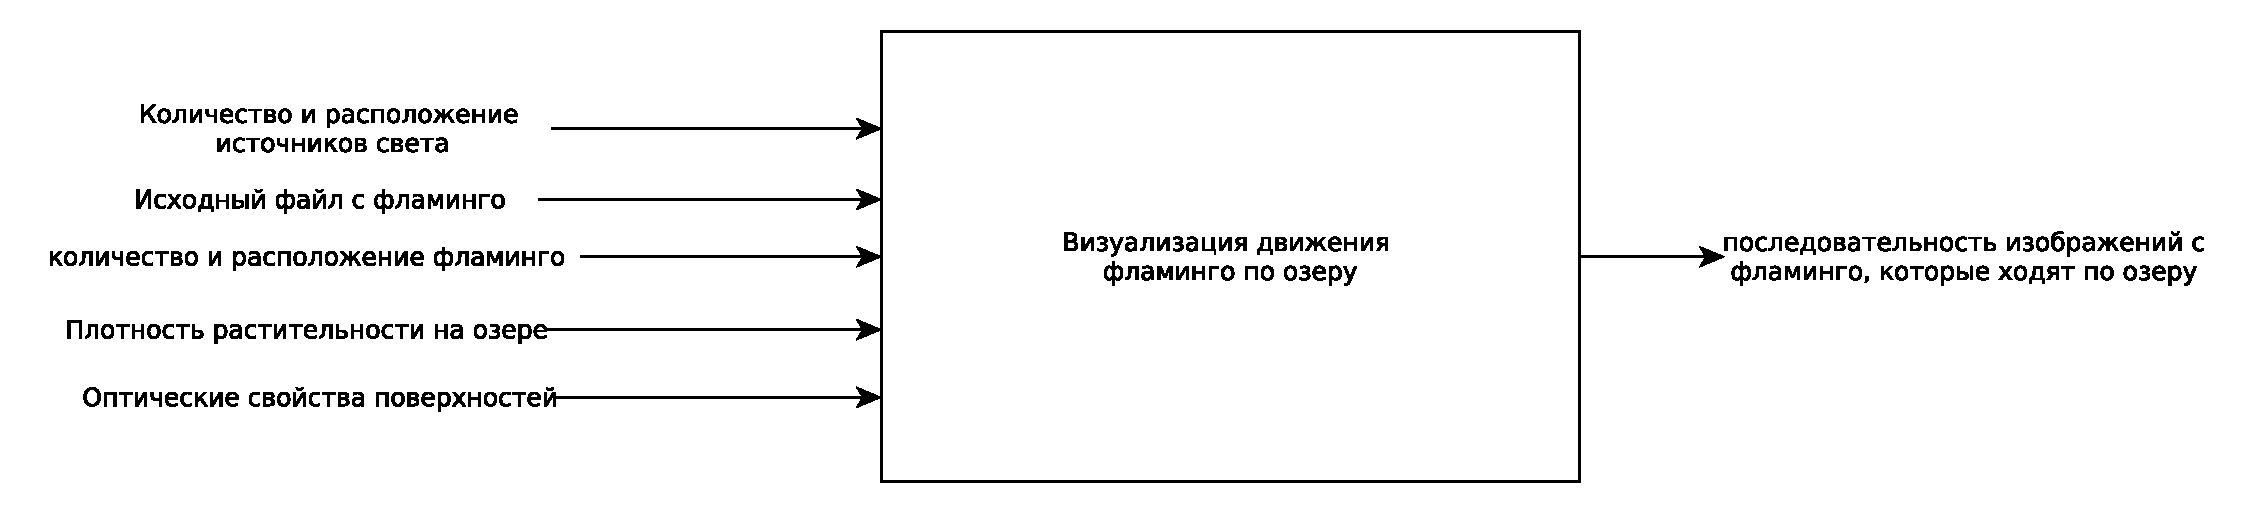
\includegraphics[width=\linewidth]{img/idef0}
	\caption{IDEF0 диаграмма, 0 уровень}
	\label{fig:idef0}
\end{figure}

\section{Требования к программному \\
	обеспечению}

К разрабатываемому программному обеспечению будут предъявлены следующие требования:
\begin{enumerate}[label=\arabic*)]
	\item наличие графического интерфейса с функционалом, который имеет возможность задать входные данные;
	\item программа принимает входные данные, учитывая ограничения, указанные выше, иначе выдает ошибку;
	\item программа может сохранять полученное изображение в файл с форматом .png;
	\item программа предоставляет возможность запустить непрерывную отрисовку кадров, чтобы можно было наблюдать ходьбу фламинго на них;
\end{enumerate} 

\section{Обзор способов задания трехмерной модели}

Модель – отображение форм и размеров объекта~\cite{kurov}.

Разделяют три вида модели: каркасная, поверхностная и твердотельная~\cite{kurov, roders, refl}.
\begin{enumerate}[label=\arabic*)]
	\item Каркасная модель. 
	
	В этой модели хранится информация только о вершинах и рёбрах объектов. Недостатком данной модели является то, что она может неправильно передавать форму объекта.
	\item Поверхностная модель.
	
	Поверхность может описываться аналитически или полигональной сеткой. Такая информационная модель содержит данные только о внешних геометрических параметрах объекта. Недостатком модели является отсутствие информации о том, с какой стороны поверхности находится материал.

	\item Твердотельная модель.
	
	При твердотельном моделировании учитывается еще и материал, из которого изготовлен объект.  С помощью указания направления внутренней нормали к информации о поверхности добавялется то, с какой стороны поверхности расположен материал.
\end{enumerate}

Для достижения поставленной цели лучше всего подходит поверхностная модель, так как она позволит достичь требуемой визуализации озера с растительностью и фламинго, не требуя большого количества вычислительных операций, как твердотельная. 

\section{Способы задания поверхностных моделей}

Существует 2 основных способа для задания поверхностной модел~\cite{roders}:
\begin{enumerate}[label=\arabic*)]
	\item Аналитический способ --- характеризуется тем, что для получения поверхности нужно дополнительно вычислять функцию, зависящую от параметра.
	
	\item Полигональная сетка --- характеризуется тем, что информация о модели хранится в виде совокупности вершин, ребер и граней.
\end{enumerate}

Из двух представленных вариантов наиболее оптимальным является использование полигональной сетки, так как такой вариант задания поверхности позволит быстро выполнять операции над объектами.


Существует несколько способов хранения полигональной сетки~\cite{roders}:
\begin{enumerate}[label=\arabic*)]
	\item Список граней --- характеризуется множеством граней и вершин. В каждую грань входят как минимум три вершины. 
	\item Вершинное представление --- характеризуется хранением информации о вершинах, которые указывают на другие вершины, с которыми они соединены.
	\item Таблица углов --- это таблица, хранящая вершины. Ее обход неявно задаёт полигоны. Такое представление занимает меньше места и более производительно для нахождения полигонов, но операции по их изменению медленные.
    \item «Крылатое» представление --- характеризуется заданием точек, каждая из которых указывает на 2 вершины, 2 грани и 4 ребра, которые ее касаются, благодаря чему обход поверхностей выполняется за постоянное время. Однако метод требует много памяти и изменения геометрических характеристик приводит к формированию списка индексов граней. Данный способ полезен для определения столкновений объектов.
\end{enumerate}

Для хранения полигональной сетки будет использоваться список граней, так как у этого способа простое и наглядное хранение информации о гранях объекта, а также этот способ обеспечивает простой доступ к геометрическим параметрам и связям с другими гранями, что упрощает операции по обходу, изменению и анализу поверхности объекта.


\section{Анализ алгоритмов удаления невидимых линий и поверхностей}

Представленные далее алгоритмы работают в одном из двух пространств: изображения или объекта~\cite{roders}. Пространство изображения --- это пространство, в котором каждая точка представляет отдельный пиксель или элемент изображения. Пространство объекта --- это пространство, в котором располагаются объекты в трехмерной форме. 

\subsection{Алгоритм, использующий $Z$-буфер}

Данный алгоритм работает в пространстве изображения~\cite{roders}.

Используются два буфера:
\begin{enumerate} [label=\arabic*)]
	\item буфер кадра, в котором хранятся атрибуты каждого пикселя в пространстве изображения;
	\item $Z$-буфер, куда помещается информация о координате $z$ для каждого пикселя.
\end{enumerate}

Пошаговое описание алгоритма Z-буфера:
\begin{enumerate} [label=\arabic*)]
	\item создаются 2 буфера: буфер кадра и буфер глубины (Z-буфер);
	\item задаются начальные значения для каждого пикселя в буфере глубины;
	\item для каждого полигона сцены вычисляется нормаль к нему;
	\item вычисляется глубина $z(x, y)$ для каждого пикселя с координатами $(x, y)$;
	\item сравнивается глубина $z(x, y)$ с глубиной $z_{buf}(x, y)$, которая хранится в буфере;
	\item если $z(x, y) < z_{buf}(x, y)$, то значение в буфере заменяется $z_{buf}(x, y) = z(x, y)$.
\end{enumerate}

Главной особенностью алгоритма является его простота реализации и высокая скорость обработки объектов. При этом использование памяти для буферов изображения для современных компьютеров является незначительным и не вызывает проблем.


\subsection{Алгоритм Робертса}


Данный алгоритм работает в пространстве объекта. Для классического алгоритма Робертса требуется, чтобы все тела были выпуклыми. Так как в ходе текущей работы нужно будет работать с невыпуклыми телами, то они предварительно должны быть разбиты на выпуклые части~\cite{roders}. 

Алгоритм состоит из 3 этапов.
\begin{enumerate} [label=\arabic*)]
	\item Во-первых, происходит подготовка исходной матрицы $V$, представляющей информацию о каждом теле. Матрица имеет размерность $4 * n$, где $n$ --- количество граней тела, и содержит коэффициенты уравнений плоскостей, проходящих через грани. 
	\item Во-вторых, выполняется удаление ребер, которые закрыты самим телом. Для этого вектор взгляда $E$ умножается на матрицу $V$, и отрицательные компоненты вектора указывают на невидимые грани.
	\item В-третьих, происходит удаление невидимых ребер, закрытых другими телами на сцене. Для определения невидимых точек ребра, строится луч, соединяющий точку наблюдения с точкой на ребре. Если луч проходит сквозь тело, то ребро невидимо.
\end{enumerate}

Главным недостатком данного алгоритма является его вычислительная сложность, которая составляет $O(n^2)$, где $n$ - количество объектов на сцене. Также все тела на сцене должны быть выпуклыми, что требует дополнительных проверок. Однако, работа в объектном пространстве и высокая сложность вычислений обеспечивают высокую точность результата.


\subsection{Алгоритм трассировки лучей}

Алгоритм работает в пространстве изображений. Основная идея заключается в анализе лучей, попадающих в наблюдателя от объектов. Однако, из-за того, что не все лучи достигают наблюдателя, было предложено рассматривать лучи в обратном направлении - от наблюдателя к объектам. Трассировка лучей включает отражение, преломление и прохождение лучей через поверхности объектов. Она завершается, когда луч пересекает поверхность непрозрачного объекта, видимого для наблюдателя~\cite{roders}.

Однако, данный метод требует множества вычислений, так как необходимо найти пересечение каждого луча с объектами сцены. Количество лучей пропорционально размеру изображения, что сказывается на производительности и скорости алгоритма. Таким образом, данный метод не подходит для решения моей задачи, где требуется быстрая отрисовка динамических сцен.

\subsection{Алгоритм Варнока}

Алгоритм Варнока оперирует в пространстве изображения и позволяет определить, какие грани или части граней объектов сцены видимы, а какие скрыты другими объектами~\cite{roders}.

Основная идея алгоритма заключается в разделении области изображения на более мелкие окна. Для каждого окна определяются связанные многоугольники, а затем определяется их видимость на сцене.

В алгоритме обычно используются выпуклые многоугольники в качестве граней, так как эффективность работы с ними выше, чем с произвольными многоугольниками.

Окно, в котором требуется отобразить сцену, должно быть прямоугольным. Алгоритм работает рекурсивно: на каждом шаге происходит анализ видимости граней, и если для определения видимости требуются дополнительные вычисления, то окно делится на 4 части, и анализ повторяется отдельно для каждой части.

Главный недостаток данного алгоритма состоит в том, что использование рекурсии может привести к большому числу шагов рекурсии и значительной вычислительной сложности.


\subsection{Вывод}

\begin{table} [] 
	\caption{Сравнение алгоритмов удаления невидимых линий}
	\label{tbl:alg_del}
	\begin{tabular}{|p{.18\textwidth}|p{.18\textwidth}|p{.18\textwidth}|p{.18\textwidth}|p{.18\textwidth}|}
		\hline
		\multirow{2}{*}{Критерии} & \multicolumn{4}{|c|}{Алгоритмы} \\
		\cline{2-5}
		& Использующий Z-буфер & Робертса & Обратной трассировки лучей & Варнока  \\
		\hline
		Основная идея & использование буфера, хранящего глубину каждого пикселя & растеризация полигонов, попиксельно сравнивается глубина полигонов и видимые растеризуются & симуляция физического взаимодействия лучей света с объектами на сцене (отражаются, преломляются или поглощаются в зависимости от свойств материалов) & растеризация полигонов, распределяются непрозрачные полигоны в порядке их удаленности от камеры и выполняется затенение полигонов в порядке удаленности \\
		\hline
		Вычислите-
		льная трудоемкость (n - кол-во граней объектов, N - кол-во пикселей)& O($N*n$) & O($n^2$) &  O($N*n$) & O($N*n$) \\		
		\hline
		Работает с невыпуклыми & да & нет & да, с доп. проверками & да, с доп. обработкой сцены\\
		\hline
		Рабочее пространство & изображение & объект & изображение & изображение \\ 
		\hline 
		Применение для сцен в реального времени & может быть эффективным, но потреблять больше памяти & используется, но может быть не эффективным для сложных сцен & обеспечивает высокое качество изображений, но может быть более затратным по времени для рендеринга сложных сцен & используется и позволяет обрабатывать большие сцены за счет эффективной сортировки и однократного прохода по полигонам \\
		\hline
	\end{tabular}
\end{table}


В качестве алгоритма удаления невидимых рёбер и поверхностей был выбран алгоритм $Z$-буфера, так как он работает в пространстве изображения и быстро производит вычисления.

\clearpage

\section{Анализ алгоритмов закраски}

Существует два наиболее распространённых метода закраски~\cite{roders}.

\subsection{Закраска Гуро}

Метод Гуро, основанный на интерполяции интенсивности, заключается в закрашивании разных точек грани с разными значениями интенсивности. Для этого вычисляется вектор нормали в каждой вершине грани, а затем значения интенсивности интерполируются по всем точкам примыкающих граней~\cite{roders}.

Закрашивание граней по методу Гуро выполняется в четыре этапа. 
\begin{enumerate} [label=\arabic*)]
	\item Вычисляются нормали к каждой грани. 
	\item Определяются нормали в вершинах, которые вычисляются как усреднение нормалей примыкающих граней. 
	\item На основе нормалей в вершинах вычисляются значения интенсивностей с учетом выбранной модели отражения света. 
	\item Полигоны граней закрашиваются цветом, соответствующим линейной интерполяции значений интенсивности в вершинах.
\end{enumerate}

Метод Гуро применим только для небольших граней, которые находятся на значительном расстоянии от источника света. Если размер грани большой, расстояние от источника света до центра грани будет меньше, чем до вершин, что должно привести к более яркой освещенности центра грани по сравнению с ребрами, но из-за линейного закона интерполяции, используемого в методе, это не удается достичь, что приводит к неестественной освещенности в некоторых участках грани.

\subsection{Закраска Фонга}

Закраска Фонга, подобно закраске Гуро, осуществляет интерполяцию, но в отличие от метода Гуро, в методе Фонга интерполируются векторы нормалей, а затем используются для определения значения интенсивности для каждой точки~\cite{kurov}.

Процесс закраски в методе Фонга включает следующие этапы:
\begin{enumerate}[label=\arabic*)]
	\item Вычисляются нормали к граням.
	\item На основе нормалей к граням определяются нормали в вершинах грани. Используя эти нормали, для каждой точки закрашиваемой грани вычисляется интерполированный вектор нормали.
	\item Направление векторов нормали используется для определения цвета точек грани в соответствии с выбранной моделью отражения света.
\end{enumerate}

Метод Фонга требует больших вычислительных затрат по сравнению с методом Гуро, однако он обеспечивает более точное приближение кривизны поверхности и, следовательно, позволяет получить более реалистичное изображение.

\subsection{Вывод}

В данной работе будет использоваться метод закраски Фонга, так как он дает наиболее реалистичное изображение, в частности зеркальных бликов.

\section{Анализ алгоритмов построения теней}

В рассмотренном алгоритме трассировки лучей, тени создаются в процессе выполнения алгоритма: пиксели затеняются, если луч пересекает объект, но не достигает источника света. 
При использовании алгоритма с $z$-буфером, для нахождения теней добавляется дополнительной теневой $z$-буфер, основанный на точке наблюдения, которая совпадает с источником света. Такая модификация позволяет избежать усложнения структуры программы и, следовательно, сократить время отладки программного продукта.

\section{Анализ моделей освещения}

Модели освещения позволяют определить, как свет будет влиять на объекты в сцене. 
Основные виды освещений представлены далее~\cite{roders}.
\begin{enumerate}[label=\arabic*)]
	\item Фоновое освещение --- это равномерное и небольшое освещение, которое создается отражением света от окружающих поверхностей. Оно дает объектам общее освещение и предотвращает полное затемнение в тени.
	\item Диффузное освещение --- это освещение, которое происходит, когда свет попадает на поверхность объекта и равномерно рассеивается во все стороны. Оно создает матовый эффект освещения и отображает интенсивность света в зависимости от угла падения на поверхность.
	\item Зеркальное освещение --- это освещение, которое создает блеск и блики на поверхности объекта. Оно происходит, когда свет падает на гладкую и отражающую поверхность, и отображает интенсивность света в зависимости от угла отражения.
\end{enumerate}

Введем следующие обозначения для коэффициентов:
\begin{itemize}
	\item $I_a$ --- интенсивность рассеянного света;
	\item $K_a$ --- коэффициент диффузного отражения рассеянного света;
	\item $I_d$ --- интенсивность диффузного освещения (diffuse),
	\item $K_d$ --- коэффициент отражения диффузного освещения,
	\item $I_s$ --- интенсивность зеркального освещения,
	\item $K_s$ --- коэффициент отражения зеркального освещения,
	\item $n$ --- бликовый коэффициент;
	\item $\vec{L}$ --- вектор от точки к источнику;
	\item $\vec{N}$ --- вектор нормали;
	\item $\vec{R}$ --- вектор отраженного луча;
	\item $\vec{V}$ --- вектор от точки к наблюдателю.
	
\end{itemize}

Коэффициенты $K_a$, $K_d$ и $K_s$ задаются отдельно для каждого материала и определяют его отражательные свойства для фонового, диффузного и зеркального освещения соответственно. Чем больше значение этих коэффициентов, тем сильнее будет отражаться соответствующий тип освещения от поверхности.

Коэффициент $n$ также определяется для каждого материала и отвечает за бликовость поверхности. Чем больше значение $n$, тем более "острые" и интенсивные будут зеркальные блики.

\subsection{Модель Ламберта}

Модель Ламберта моделирует диффузное освещение~\cite{roders}.

Свет от точечного источника отражается по закону Ламберта~(\ref{for:lambert}). 

\begin{equation}
	\label{for:lambert}
	I = I_i \cdot k_d \cdot (\vec{L}, \vec{N}),
\end{equation}

Модель Ламберта является простой в реализации моделью, однако основной недостаток --- одинаковая интенсивность во всех точках, принадлежащих одной грани.


\subsection{Модель Фонга}

Модель Фонга является моделью освещения, которая комбинирует фоновое освещение с диффузной и зеркальной составляющими. Благодаря зеркальному отражению на блестящих предметах появляются световые блики~\cite{roders}.

Коэффициент зеркального отражения зависит от угла падения, однако даже при перпендикулярном падении зеркально отражается только часть света, а остальное либо поглощается, либо отражается диффузно. Эти соотношения определяются свойствами вещества и длиной волны. Объединяя эти результаты с формулой рассеянного света и диффузного отражения, получим модель освещения~(\ref{for:phong1}).
\begin{equation} 
	\label{for:phong1}
	I = I_a * K_a + I_d * K_d * (\vec{L} \cdot \vec{N}) + I_s * K_s * (\vec{R} \cdot \vec{V})^n,
\end{equation}

\subsection{Вывод}

Была выбрана модель освещения Фонга, так как была поставлена задача реалистичной визуализации, а для нее нужно не только диффузное освещение, как в модели Ламберта.


\section{Итоговый выбор алгоритмов} 

Для задания трёхмерных моделей была выбрана поверхностная модель, она будет задаваться полигональной сеткой. В качестве алгоритма удаления невидимых линий был выбран алгоритм, использующий $Z$-буфер, построение теней будет выполняться с помощью модифицированного алгоритма z-буфера, освещение и закраска с помощью алгоритма Фонга.

